% (find-LATEX "2020-2-C2-P1.tex")
% (defun c () (interactive) (find-LATEXsh "lualatex -record 2020-2-C2-P1.tex" :end))
% (defun C () (interactive) (find-LATEXsh "lualatex 2020-2-C2-P1.tex" "Success!!!"))
% (defun D () (interactive) (find-pdf-page      "~/LATEX/2020-2-C2-P1.pdf"))
% (defun d () (interactive) (find-pdftools-page "~/LATEX/2020-2-C2-P1.pdf"))
% (defun e () (interactive) (find-LATEX "2020-2-C2-P1.tex"))
% (defun o () (interactive) (find-LATEX "2020-2-C2-P1.tex"))
% (defun u () (interactive) (find-latex-upload-links "2020-2-C2-P1"))
% (defun v () (interactive) (find-2a '(e) '(d)))
% (defun d0 () (interactive) (find-ebuffer "2020-2-C2-P1.pdf"))
% (defun cv () (interactive) (C) (ee-kill-this-buffer) (v) (g))
%          (code-eec-LATEX "2020-2-C2-P1")
% (find-pdf-page   "~/LATEX/2020-2-C2-P1.pdf")
% (find-sh0 "cp -v  ~/LATEX/2020-2-C2-P1.pdf /tmp/")
% (find-sh0 "cp -v  ~/LATEX/2020-2-C2-P1.pdf /tmp/pen/")
%     (find-xournalpp "/tmp/2020-2-C2-P1.pdf")
%   file:///home/edrx/LATEX/2020-2-C2-P1.pdf
%               file:///tmp/2020-2-C2-P1.pdf
%           file:///tmp/pen/2020-2-C2-P1.pdf
% http://angg.twu.net/LATEX/2020-2-C2-P1.pdf
% (find-LATEX "2019.mk")
% (find-CN-aula-links "2020-2-C2-P1" "2" "c2m202p1" "c2p1")
%
% Video:
% (find-ssr-links "c2m202p1" "2020-2-C2-P1")
% (code-video     "c2m202p1video" "$S/http/angg.twu.net/eev-videos/2020-2-C2-P1.mp4")
% (find-c2m202p1video "0:00")

% «.defs»		(to "defs")
% «.title»		(to "title")
% «.regras-e-dicas»	(to "regras-e-dicas")
% «.questao-1»		(to "questao-1")
% «.questao-2»		(to "questao-2")
% «.questao-3»		(to "questao-3")
% «.questao-4»		(to "questao-4")
% «.gabarito-1»		(to "gabarito-1")
% «.gabarito-2»		(to "gabarito-2")
% «.gabarito-3»		(to "gabarito-3")
% «.gabarito-4»		(to "gabarito-4")
%
% «.djvuize»	(to "djvuize")

\documentclass[oneside,12pt]{article}
\usepackage[colorlinks,citecolor=DarkRed,urlcolor=DarkRed]{hyperref} % (find-es "tex" "hyperref")
\usepackage{amsmath}
\usepackage{amsfonts}
\usepackage{amssymb}
\usepackage{pict2e}
\usepackage[x11names,svgnames]{xcolor} % (find-es "tex" "xcolor")
\usepackage{colorweb}                  % (find-es "tex" "colorweb")
%\usepackage{tikz}
%
% (find-dn6 "preamble6.lua" "preamble0")
%\usepackage{proof}   % For derivation trees ("%:" lines)
%\input diagxy        % For 2D diagrams ("%D" lines)
%\xyoption{curve}     % For the ".curve=" feature in 2D diagrams
%
\usepackage{edrx15}               % (find-LATEX "edrx15.sty")
\input edrxaccents.tex            % (find-LATEX "edrxaccents.tex")
\input edrxchars.tex              % (find-LATEX "edrxchars.tex")
\input edrxheadfoot.tex           % (find-LATEX "edrxheadfoot.tex")
\input edrxgac2.tex               % (find-LATEX "edrxgac2.tex")
%
%\usepackage[backend=biber,
%   style=alphabetic]{biblatex}            % (find-es "tex" "biber")
%\addbibresource{catsem-slides.bib}        % (find-LATEX "catsem-slides.bib")
%
% (find-es "tex" "geometry")
\usepackage[a6paper, landscape,
            top=1.5cm, bottom=.25cm, left=1cm, right=1cm, includefoot
           ]{geometry}
%
\begin{document}

\catcode`\^^J=10
\directlua{dofile "dednat6load.lua"}  % (find-LATEX "dednat6load.lua")

%L dofile "edrxtikz.lua"  -- (find-LATEX "edrxtikz.lua")
%L dofile "edrxpict.lua"  -- (find-LATEX "edrxpict.lua")
\pu

% «defs»  (to ".defs")
% (find-LATEX "edrx15.sty" "colors-2019")
\long\def\ColorRed   #1{{\color{Red1}#1}}
\long\def\ColorViolet#1{{\color{MagentaVioletLight}#1}}
\long\def\ColorViolet#1{{\color{Violet!50!black}#1}}
\long\def\ColorGreen #1{{\color{SpringDarkHard}#1}}
\long\def\ColorGreen #1{{\color{SpringGreenDark}#1}}
\long\def\ColorGreen #1{{\color{SpringGreen4}#1}}
\long\def\ColorGray  #1{{\color{GrayLight}#1}}
\long\def\ColorGray  #1{{\color{black!30!white}#1}}
\long\def\ColorBrown #1{{\color{Brown}#1}}
\long\def\ColorBrown #1{{\color{brown}#1}}
\long\def\ColorOrange#1{{\color{orange}#1}}

\long\def\ColorShort #1{{\color{SpringGreen4}#1}}
\long\def\ColorLong  #1{{\color{Red1}#1}}

\def\frown{\ensuremath{{=}{(}}}
\def\True {\mathbf{V}}
\def\False{\mathbf{F}}
\def\D    {\displaystyle}

\def\drafturl{http://angg.twu.net/LATEX/2020-2-C2.pdf}
\def\drafturl{http://angg.twu.net/2020.2-C2.html}
\def\draftfooter{\tiny \href{\drafturl}{\jobname{}} \ColorBrown{\shorttoday{} \hours}}



%  _____ _ _   _                               
% |_   _(_) |_| | ___   _ __   __ _  __ _  ___ 
%   | | | | __| |/ _ \ | '_ \ / _` |/ _` |/ _ \
%   | | | | |_| |  __/ | |_) | (_| | (_| |  __/
%   |_| |_|\__|_|\___| | .__/ \__,_|\__, |\___|
%                      |_|          |___/      
%
% «title»  (to ".title")
% (c2m202p1p 1 "title")
% (c2m202p1    "title")

\thispagestyle{empty}

\begin{center}

\vspace*{1.2cm}

{\bf \Large Cálculo 2 - 2020.2}

\bsk

P1 (primeira prova)

\bsk

Eduardo Ochs - RCN/PURO/UFF

\url{http://angg.twu.net/2020.2-C2.html}

\end{center}

\newpage

% «regras-e-dicas»  (to ".regras-e-dicas")
% (c2m202p1p 2 "regras-e-dicas")
% (c2m202p1    "regras-e-dicas")

As regras e dicas são as mesmas dos mini-testes:

\ssk

\url{http://angg.twu.net/LATEX/2020-2-C2-MT1.pdf}

\url{http://angg.twu.net/LATEX/2020-2-C2-MT2.pdf}

\ssk

exceto que a prova vai ser disponibilizada às 17:00 do dia

15/abril/2021 e deve ser entregue até as 20:00 do dia

16/abril/2021.

\newpage

% «questao-1»  (to ".questao-1")
% (c2m202p1p 3 "questao-1")
% (c2m202p1    "questao-1")

{\bf Questão 1}

(Total: 2.5pts)

\ssk

Sejam:
%
$$f(x) =
  \begin{cases}
  1 & \text{se $x≤1$}, \\
  2 & \text{se $1<x$}, \\
  \end{cases}
  \qquad
  F(x) =
  \begin{cases}
  x & \text{se $x≤1$}, \\
  2x & \text{se $1<x$}. \\
  \end{cases}
$$

a) Desenhe os gráficos das funções $f(x)$ e $F(x)$.

b) É verdade que $F'(x)=f(x)$?

c) É verdade que $F$ é uma primitiva de $f$?

\ssk

d) É verdade que $\D \Intx{0}{2}{f(x)} = \Difx{0}{2}{F(x)}$?

\newpage

% «questao-2»  (to ".questao-2")
% (c2m202p1p 4 "questao-2")
% (c2m202p1    "questao-2")
% (c2m202mt2p 4 "questao")
% (c2m202mt2    "questao")

{\bf Questão 2}

(Total: 2.5pts)

\ssk

{\sl Toda integral que pode ser resolvida por uma sequência de
  mudanças de variável (ou: ``por uma sequência de integrações por
  substituição'') pode ser resolvida por uma mudança de variável só.}
Vocês viram isso no mini-teste: a integral dele podia ser resolvida
usando as duas mudanças de variável $[u = \sqrt{x}]$ e $[v = 2u + 3]$
ou usando só $[w = 2\sqrt{x} + 3]$.

Resolva a integral abaixo de dois jeitos diferentes:
%
$$\intx {\frac{3 \cos{\left (2 + \sqrt{3 x + 4} \right )}}
         {2 \sqrt{3 x + 4}}
        }
$$

a) por várias mudanças simples de variável,

b) por uma mudança de variável só.






\newpage

% «questao-3»  (to ".questao-3")
% (c2m202p1p 5 "questao-3")
% (c2m202p1    "questao-3")

{\bf Questão 3}

(Total: 2.5pts)

\ssk

Um dos exercícios dos slides de frações parciais pedia pra vocês
integrarem $\intx{\frac 1{3x}}$. Tem dois jeitos de fazer essa conta,
um começando com $\intx{\frac 1{3x}} = \frac 13 \intx{\frac 1x}$ e
outro começando com a substituição $[u=3x]$, e os dois dão resultados
diferentes. Faça as contas, entenda os detalhes, e explique o porquê
desses dois resultados diferentes imaginando que você está explicando
pra alguém que acabou de aprender integração por substituição mas
ainda não tem muita prática.

\newpage

% «questao-4»  (to ".questao-4")
% (c2m202p1p 6 "questao-4")
% (c2m202p1    "questao-4")

{\bf Questão 4}

(Total: 2.5pts)

\ssk

Integre
%
$$\intth{\frac{\senθ}{\cosθ}}$$

e teste a sua resposta.

\msk

Dica: use um dos jeitos de integrar potências de senos e cossenos

e depois use a regra da potência.



\newpage

\thispagestyle{empty}

\begin{center}

\vspace*{2.0cm}

{\bf \Large Gabarito}

(incompleto)

\end{center}


\newpage

% «gabarito-1»  (to ".gabarito-1")
% (c2m202p1p 8 "gabarito-1")
% (c2m202p1    "gabarito-1")

{\bf Questão 1: gabarito}

\msk

a) 
$\qquad
 f(x) \;\; = \;\;
 \vcenter{\hbox{%
 \unitlength=10pt
 \beginpicture(0,0)(2,4)
   \pictgrid%
   \pictpiecewise{(0,1)--(1,1)c
                  (1,2)o--(2,2)
                  }%
   \pictaxes%
 \end{picture}%
 }}
 \qquad
 F(x) \;\; = \;\;
 \vcenter{\hbox{%
 \unitlength=10pt
 \beginpicture(0,0)(2,4)
   \pictgrid%
   \pictpiecewise{(0,0)--(1,1)c
                  (1,2)o--(2,4)
                  }%
   \pictaxes%
 \end{picture}%
 }}
$

\msk

b) Isto é falso em $x=1$: $f(1)=1$ mas $F'(1)$ não existe.

c) Não. Veja a definição:

% (c2m202escadasp 16 "exercicio-8")
% (c2m202escadas     "exercicio-8")
% http://angg.twu.net/LATEX/2020-2-C2-escadas.pdf#page=16
\url{http://angg.twu.net/LATEX/2020-2-C2-escadas.pdf\#page=16}

\msk

d) Não: $3 = \D \Intx{0}{2}{f(x)} \neq \Difx{0}{2}{F(x)} = 4$.

\newpage

% «gabarito-2»  (to ".gabarito-2")
% (c2m202p1p 9 "gabarito-2")
% (c2m202p1    "gabarito-2")

{\bf Questão 2: gabarito}

\msk

$\scalebox{0.85}{$
 \begin{array}{l}
   \begin{array}{l}
   \intx {\frac{3 \cos{\left (2 + \sqrt{3 x + 4} \right )}}
         {2 \sqrt{3 x + 4}}
         } \\
   = \intu {\frac{\cos{\left (2 + \sqrt{u + 4} \right )}}
           {2 \sqrt{u + 4}}
           } \\
   = \intv {\frac{\cos{\left (2 + \sqrt{v} \right )}}
           {2 \sqrt{v}}
           } \\
   = \intw {\cos{\left (2 + w \right )}
           } \\
   = \inty {\cos y}
           \\
   = \sen y \\
   = \sen \left( 2+w \right) \\
   = \sen \left( 2+\sqrt{v} \right) \\
   = \sen \left( 2+\sqrt{u+4} \right) \\
   = \sen \left( 2+\sqrt{3x+4} \right) \\
   \end{array}
   %
   \begin{array}{c}
     \bsm{u = 3x \\ \frac{du}{dx} = 3 \\ du = 3\,dx \\ dx = \frac13 du}
     \\[15pt]
     \bsm{v = u+4 \\ du=dv }
     \\[5pt]
     \bsm{w = \sqrt{v} \\ \frac{dw}{dv} = \frac12 v^{-1/2} = \frac{1}{2\sqrt{v}} \\}
     \\[5pt]
     \bsm{y = 2+w \\ dy=dw }
     \\[60pt]
   \end{array}
   %
   \\
   \\
   %
   \begin{array}{l}
   \intx {\frac{3 \cos{\left (2 + \sqrt{3 x + 4} \right )}}
         {2 \sqrt{3 x + 4}}
         } \\
   = \intu {\cos u} \\
   = \sen u \\
   = \sen \left( 2 + \sqrt{3x+4} \right) \\
   \end{array}
   %
   \begin{array}{c}
     \bsm{u = 2 + \sqrt{3x+4} \\
          \frac{du}{dx} = \frac{3}{2 \sqrt{3 x + 4}} \\
         }
     \\[15pt]
   \end{array}
 %
 \end{array}
 $}
$


\newpage

% «gabarito-3»  (to ".gabarito-3")
% (c2m202p1p 10 "gabarito-3")
% (c2m202p1     "gabarito-3")
% http://angg.twu.net/LATEX/2020-2-C2-P1.pdf#page=10
% (find-fline "~/2020.2-C2/tmp/")
% (find-fline "~/2020.2-C2/tmp/20210408_C2_P1_gab_3.jpg")

{\bf Questão 3: gabarito}

$$\begin{array}{l}
  \intx{\frac{1}{3x}} \\
  = \intu{\frac{1}{u}·\frac13} \\
  = \frac13 \intu{\frac{1}{u}} \\
  = \frac13 \ln u \\
  = \frac13 \ln(3x) \\
  \end{array}
  %
  \bmat{
  u = 3x \\ x = \frac13 u \\ dx = \frac13 du
  }
  %
  \qquad
  \qquad
  %
  \begin{array}{l}
  \intx{\frac{1}{3x}} \\
  = \frac13 \intx{\frac{1}{x}} \\
  = \frac13 \ln x \\
  \\
  \\
  \end{array}
  %
$$

$$\begin{array}{l}
  \frac13 \ln(3x) \\
  = \frac13 ((\ln3) + (\ln x)) \\
  = (\frac13 \ln3) + (\frac13\ln x) \\
  \end{array}
$$

\bsk

As duas integrais que obtivemos
para $\frac{1}{3x}$

diferem por uma constante.

% (find-latexscan-links "C2" "20210408_C2_P1_gab_3")
% (find-xpdf-page "~/LATEX/2020-2-C2/20210408_C2_P1_gab_3.pdf")
%\includegraphics[height=7cm]{2020-2-C2/20210408_C2_P1_gab_3.pdf}


\newpage

% «gabarito-4»  (to ".gabarito-4")
% (c2m202p1p 11 "gabarito-4")
% (c2m202p1     "gabarito-4")
% (find-fline "~/2020.2-C2/tmp/20210419_C2_P1_gab_4.jpg")

{\bf Questão 4: gabarito}

% (find-latexscan-links "C2" "20210419_C2_P1_gab_4")
% (find-xpdf-page "~/LATEX/2020-2-C2/20210419_C2_P1_gab_4.pdf")
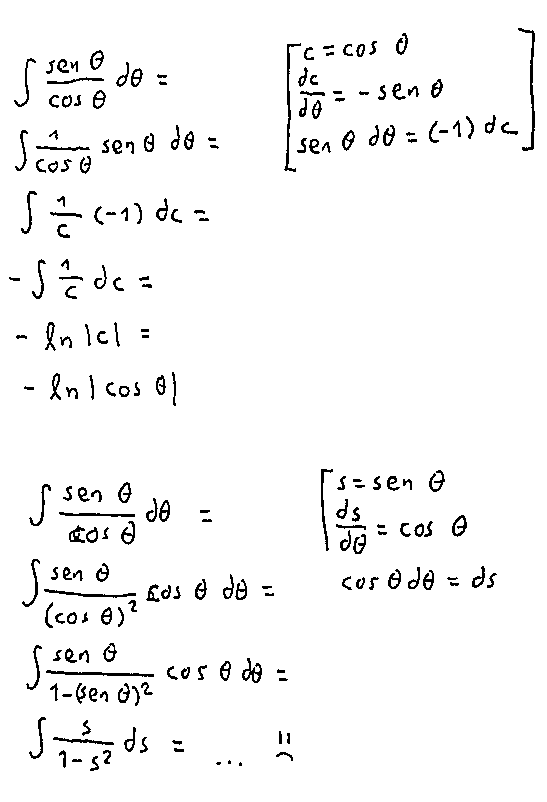
\includegraphics[height=7cm]{2020-2-C2/20210419_C2_P1_gab_4.pdf}





%\printbibliography

\GenericWarning{Success:}{Success!!!}  % Used by `M-x cv'

\end{document}

%  ____  _             _         
% |  _ \(_)_   ___   _(_)_______ 
% | | | | \ \ / / | | | |_  / _ \
% | |_| | |\ V /| |_| | |/ /  __/
% |____// | \_/  \__,_|_/___\___|
%     |__/                       
%
% «djvuize»  (to ".djvuize")
% (find-LATEXgrep "grep --color -nH --null -e djvuize 2020-1*.tex")

 (eepitch-shell)
 (eepitch-kill)
 (eepitch-shell)
# (find-fline "~/2020.2-C2/")
# (find-fline "~/LATEX/2020-2-C2/")
# (find-fline "~/bin/djvuize")

cd /tmp/
for i in *.jpg; do echo f $(basename $i .jpg); done

f () { rm -fv $1.png $1.pdf; djvuize $1.pdf }
f () { rm -fv $1.png $1.pdf; djvuize WHITEBOARDOPTS="-m 1.0" $1.pdf; xpdf $1.pdf }
f () { rm -fv $1.png $1.pdf; djvuize WHITEBOARDOPTS="-m 0.5" $1.pdf; xpdf $1.pdf }
f () { rm -fv $1.png $1.pdf; djvuize WHITEBOARDOPTS="-m 0.25" $1.pdf; xpdf $1.pdf }
f () { cp -fv $1.png $1.pdf       ~/2020.2-C2/
       cp -fv        $1.pdf ~/LATEX/2020-2-C2/
       cat <<%%%
% (find-latexscan-links "C2" "$1")
%%%
}

f 20210408_C2_P1_gab_3
f 20210419_C2_P1_gab_4



%  __  __       _        
% |  \/  | __ _| | _____ 
% | |\/| |/ _` | |/ / _ \
% | |  | | (_| |   <  __/
% |_|  |_|\__,_|_|\_\___|
%                        
% <make>

 (eepitch-shell)
 (eepitch-kill)
 (eepitch-shell)
# (find-LATEXfile "2019planar-has-1.mk")
make -f 2019.mk STEM=2020-2-C2-P1 veryclean
make -f 2019.mk STEM=2020-2-C2-P1 pdf

% Local Variables:
% coding: utf-8-unix
% ee-tla: "c2m202p1"
% End:
